\documentclass[]{book}
\usepackage{lmodern}
\usepackage{amssymb,amsmath}
\usepackage{ifxetex,ifluatex}
\usepackage{fixltx2e} % provides \textsubscript
\ifnum 0\ifxetex 1\fi\ifluatex 1\fi=0 % if pdftex
  \usepackage[T1]{fontenc}
  \usepackage[utf8]{inputenc}
\else % if luatex or xelatex
  \ifxetex
    \usepackage{mathspec}
  \else
    \usepackage{fontspec}
  \fi
  \defaultfontfeatures{Ligatures=TeX,Scale=MatchLowercase}
\fi
% use upquote if available, for straight quotes in verbatim environments
\IfFileExists{upquote.sty}{\usepackage{upquote}}{}
% use microtype if available
\IfFileExists{microtype.sty}{%
\usepackage{microtype}
\UseMicrotypeSet[protrusion]{basicmath} % disable protrusion for tt fonts
}{}
\usepackage[margin=1in]{geometry}
\usepackage{hyperref}
\hypersetup{unicode=true,
            pdftitle={Spatial Statistics for Stream Networks},
            pdfauthor={Jay M. Ver Hoef, Erin E. Peterson, Daniel J. Isaak},
            pdfborder={0 0 0},
            breaklinks=true}
\urlstyle{same}  % don't use monospace font for urls
\usepackage{natbib}
\bibliographystyle{apalike}
\usepackage{color}
\usepackage{fancyvrb}
\newcommand{\VerbBar}{|}
\newcommand{\VERB}{\Verb[commandchars=\\\{\}]}
\DefineVerbatimEnvironment{Highlighting}{Verbatim}{commandchars=\\\{\}}
% Add ',fontsize=\small' for more characters per line
\usepackage{framed}
\definecolor{shadecolor}{RGB}{248,248,248}
\newenvironment{Shaded}{\begin{snugshade}}{\end{snugshade}}
\newcommand{\AlertTok}[1]{\textcolor[rgb]{0.94,0.16,0.16}{#1}}
\newcommand{\AnnotationTok}[1]{\textcolor[rgb]{0.56,0.35,0.01}{\textbf{\textit{#1}}}}
\newcommand{\AttributeTok}[1]{\textcolor[rgb]{0.77,0.63,0.00}{#1}}
\newcommand{\BaseNTok}[1]{\textcolor[rgb]{0.00,0.00,0.81}{#1}}
\newcommand{\BuiltInTok}[1]{#1}
\newcommand{\CharTok}[1]{\textcolor[rgb]{0.31,0.60,0.02}{#1}}
\newcommand{\CommentTok}[1]{\textcolor[rgb]{0.56,0.35,0.01}{\textit{#1}}}
\newcommand{\CommentVarTok}[1]{\textcolor[rgb]{0.56,0.35,0.01}{\textbf{\textit{#1}}}}
\newcommand{\ConstantTok}[1]{\textcolor[rgb]{0.00,0.00,0.00}{#1}}
\newcommand{\ControlFlowTok}[1]{\textcolor[rgb]{0.13,0.29,0.53}{\textbf{#1}}}
\newcommand{\DataTypeTok}[1]{\textcolor[rgb]{0.13,0.29,0.53}{#1}}
\newcommand{\DecValTok}[1]{\textcolor[rgb]{0.00,0.00,0.81}{#1}}
\newcommand{\DocumentationTok}[1]{\textcolor[rgb]{0.56,0.35,0.01}{\textbf{\textit{#1}}}}
\newcommand{\ErrorTok}[1]{\textcolor[rgb]{0.64,0.00,0.00}{\textbf{#1}}}
\newcommand{\ExtensionTok}[1]{#1}
\newcommand{\FloatTok}[1]{\textcolor[rgb]{0.00,0.00,0.81}{#1}}
\newcommand{\FunctionTok}[1]{\textcolor[rgb]{0.00,0.00,0.00}{#1}}
\newcommand{\ImportTok}[1]{#1}
\newcommand{\InformationTok}[1]{\textcolor[rgb]{0.56,0.35,0.01}{\textbf{\textit{#1}}}}
\newcommand{\KeywordTok}[1]{\textcolor[rgb]{0.13,0.29,0.53}{\textbf{#1}}}
\newcommand{\NormalTok}[1]{#1}
\newcommand{\OperatorTok}[1]{\textcolor[rgb]{0.81,0.36,0.00}{\textbf{#1}}}
\newcommand{\OtherTok}[1]{\textcolor[rgb]{0.56,0.35,0.01}{#1}}
\newcommand{\PreprocessorTok}[1]{\textcolor[rgb]{0.56,0.35,0.01}{\textit{#1}}}
\newcommand{\RegionMarkerTok}[1]{#1}
\newcommand{\SpecialCharTok}[1]{\textcolor[rgb]{0.00,0.00,0.00}{#1}}
\newcommand{\SpecialStringTok}[1]{\textcolor[rgb]{0.31,0.60,0.02}{#1}}
\newcommand{\StringTok}[1]{\textcolor[rgb]{0.31,0.60,0.02}{#1}}
\newcommand{\VariableTok}[1]{\textcolor[rgb]{0.00,0.00,0.00}{#1}}
\newcommand{\VerbatimStringTok}[1]{\textcolor[rgb]{0.31,0.60,0.02}{#1}}
\newcommand{\WarningTok}[1]{\textcolor[rgb]{0.56,0.35,0.01}{\textbf{\textit{#1}}}}
\usepackage{longtable,booktabs}
\usepackage{graphicx,grffile}
\makeatletter
\def\maxwidth{\ifdim\Gin@nat@width>\linewidth\linewidth\else\Gin@nat@width\fi}
\def\maxheight{\ifdim\Gin@nat@height>\textheight\textheight\else\Gin@nat@height\fi}
\makeatother
% Scale images if necessary, so that they will not overflow the page
% margins by default, and it is still possible to overwrite the defaults
% using explicit options in \includegraphics[width, height, ...]{}
\setkeys{Gin}{width=\maxwidth,height=\maxheight,keepaspectratio}
\IfFileExists{parskip.sty}{%
\usepackage{parskip}
}{% else
\setlength{\parindent}{0pt}
\setlength{\parskip}{6pt plus 2pt minus 1pt}
}
\setlength{\emergencystretch}{3em}  % prevent overfull lines
\providecommand{\tightlist}{%
  \setlength{\itemsep}{0pt}\setlength{\parskip}{0pt}}
\setcounter{secnumdepth}{5}
% Redefines (sub)paragraphs to behave more like sections
\ifx\paragraph\undefined\else
\let\oldparagraph\paragraph
\renewcommand{\paragraph}[1]{\oldparagraph{#1}\mbox{}}
\fi
\ifx\subparagraph\undefined\else
\let\oldsubparagraph\subparagraph
\renewcommand{\subparagraph}[1]{\oldsubparagraph{#1}\mbox{}}
\fi

%%% Use protect on footnotes to avoid problems with footnotes in titles
\let\rmarkdownfootnote\footnote%
\def\footnote{\protect\rmarkdownfootnote}

%%% Change title format to be more compact
\usepackage{titling}

% Create subtitle command for use in maketitle
\newcommand{\subtitle}[1]{
  \posttitle{
    \begin{center}\large#1\end{center}
    }
}

\setlength{\droptitle}{-2em}

  \title{Spatial Statistics for Stream Networks}
    \pretitle{\vspace{\droptitle}\centering\huge}
  \posttitle{\par}
    \author{Jay M. Ver Hoef, Erin E. Peterson, Daniel J. Isaak}
    \preauthor{\centering\large\emph}
  \postauthor{\par}
      \predate{\centering\large\emph}
  \postdate{\par}
    \date{2018-11-18}

\usepackage{booktabs}
\usepackage{amsthm}
\makeatletter
\def\thm@space@setup{%
  \thm@preskip=8pt plus 2pt minus 4pt
  \thm@postskip=\thm@preskip
}
\makeatother

\usepackage{amsthm}
\newtheorem{theorem}{Theorem}[chapter]
\newtheorem{lemma}{Lemma}[chapter]
\theoremstyle{definition}
\newtheorem{definition}{Definition}[chapter]
\newtheorem{corollary}{Corollary}[chapter]
\newtheorem{proposition}{Proposition}[chapter]
\theoremstyle{definition}
\newtheorem{example}{Example}[chapter]
\theoremstyle{definition}
\newtheorem{exercise}{Exercise}[chapter]
\theoremstyle{remark}
\newtheorem*{remark}{Remark}
\newtheorem*{solution}{Solution}
\begin{document}
\maketitle

{
\setcounter{tocdepth}{1}
\tableofcontents
}
\hypertarget{preface}{%
\chapter*{Preface}\label{preface}}
\addcontentsline{toc}{chapter}{Preface}

This book is a result of a long collaboration among the three of us. Our
journey began at the \emph{Holiday Inn Express on the River} in
Corvallis, Oregon, in August of 2003. Jay was on a review committee for
the
\href{https://cfpub.epa.gov/ncer_abstracts/index.cfm/fuseaction/display.abstractDetail/abstract/7821/report/0}{EPA
STARMAP grant} to Oregon State University and Colorado State University.
Erin was working on her Ph.D.~with Dave Theobald at Colorado State
University, and they were doing research on the grant. Erin and Dave had
presented some of their research. Later, some of us who had travelled to
Corvallis, were on the deck of the Holiday Inn overlooking the
Willamette River, relaxing with a drink. Erin and Dave posed the
question to Jay, ``We would like to do kriging on streams, but use
stream distance, rather than Euclidean distance. Is it possible?''

Jay has used spatial moving averages (also called process convolutions),
on several previous publications, to develop flexible spatial covariance
models, and for multivariable models. He had thought about the
possibility of using these models on other topologies, even specifically
stream networks. However, the task of getting data into a Geographical
Information System (GIS), and extracting the necessary information, was
daunting, and he had no one pressing him with a real application. Erin
and Dave provided the necessary push, and they had extensive GIS
experience. The collaboration was initiated.

About a year later, Jay taught a course on Spatial Statistics with Noel
Cressie in Switzerland. While soaking in the spa at Yverdon les Bains,
Jay explained his work on stream networks to Noel. Noel then worked with
his colleagues, specifically Bronwyn Harch, and used these ideas for
some research they had on stream networks in Australia. The two seminal
papers appeared

\hypertarget{software}{%
\section*{Software}\label{software}}
\addcontentsline{toc}{section}{Software}

The \textbf{SSN} package can be installed from CRAN. In an \textbf{R}
terminal type

\begin{Shaded}
\begin{Highlighting}[]
\KeywordTok{install.packages}\NormalTok{(}\StringTok{"SSN"}\NormalTok{)}
\end{Highlighting}
\end{Shaded}

\hypertarget{intro}{%
\chapter{Introduction}\label{intro}}

Spatial statistical models are broadly applied within the fields of
geology, geography, ecology, real estate, and medicine, just to name a
few. Spatial statistical models often have two broad goals: 1) to
describe how covariates affect a response variable, and 2) to make
predictions at unsampled locations. For example, data might be used to
fit a model establishing a relationship between elevation and air
temperature, and also to make a map of air temperature based on a dense
set of predictions. When fitting the model and making predictions, a
spatial statistical model uses a covariance matrix composed of
autocovariance values that rely on Euclidean distances (from straight
lines in two dimensions) among all sites. Distances for stream networks,
however, are poorly represented by Euclidean distances because fish and
water quality attributes do not move over land but follow the sinuous
pattern of the network. To apply traditional spatial statistical
modeling techniques, those distances must be accurately represented in a
covariance matrix structure for stream networks. This chapter provides
an overview of recent research on this topic and a new class of
spatial-stream network (SSN) model that is being used for an increasing
number of applications.

\citet{Ver:Pete:Theo:spat:2006} and
\citet{Cres:Frey:Harc:Smit:spat:2006} initially described new models for
stream networks based on moving average constructions. The models used
stream distance, which was defined as the shortest distance between two
locations computed only along the stream network.
\citep{Pete:Theo:Ver:supp:2007} provide in-depth discussion on the
statistical and ecological consequences of substituting stream distance
measures for Euclidean distance. The original work defined a class where
the moving average function was termed ``tail-up,'' and further models
with a ``tail-down'' moving average function were described by
\citep{Ver:Pete:Move:2010}, and we give further details below. Both
types of models were necessary to cover a range of autocorrelation
possibilities, so a variance component approach, combining tail-up,
tail-down, and classical geostatistical models based on Euclidean
distance, was promoted in \citet{Garr:Mone:Ver:spat:2009},
\citet{Pete:Ver:mixe:2010} and \citet{Ver:Pete:Move:2010}. Although SSN
models are most often used for streams, they can be generalized to other
dendritic networks \citep{Pete:Ver:Isaa:stre:2013}.

Because each stream topology is unique, prior to fitting the SSN models,
data are preprocessed to develop distance and weighting matrices in a
geographical information system (GIS) using the STARS (Spatial Tools for
the Analysis of River Systems) custom toolset \citep{Pete:Ver:STAR:2014}
for ArcGIS \citep{ESRI:ArcG:2014}. STARS produces the spatial,
topological, and attribute information needed to fit a SSN model using
the \textbf{SSN} package \citep{Ver:Pete:Clif:Shah:SSN:2014} with the
\textbf{R} statistical software \citep{R:Deve:Core:ALan:2015}.

New spatial statistical methods were recently developed to fit models to
data collected on stream (river) networks \citep{Ver:Pete:Move:2010}.
Stream networks, in our usage, are based on a mathematical topology that
represents streams as line segments that converge downstream, or viewed
conversely, that create dichotomous branching when moving upstream from
an outlet (the most downstream location in the network). A number of
packages (including, but not limited to, \textbf{geoR}
\citep{Ribe:Digg:geoR:2001}, \textbf{spatial}
\citep{Vene:Ripl:mode:2002}, \textbf{geoRglm}
\citep{Chri:Ribe:geoR:2002}, \textbf{gstat} \citep{Pebe:mult:2004},
\textbf{fields} \citep{Fiel:Deve:Team:2006}, \textbf{spBayes}
\citep{Finl:Bane:Carl:spBa:2007}, and \textbf{ramps}
\citep{Smit:Yan:Cowl:unif:2008}) have been written in \textbf{R} to fit
spatial statistical models that use geostatistical autocovariance
functions (based on Euclidean distance), but they are not guaranteed to
produce positive-definite covariance matrices when using an alternative
distance measure, such as stream distance
\citep{Ver:Pete:Theo:spat:2006}. In this book, we present the \textbf{R}
package \textbf{SSN}, which allows users to fit autocovariance functions
developed for stream networks \citep{Ver:Pete:Move:2010}. These models
are unique because they use distance measured along the network, they
incorporate flow direction, and they allow covariance weighting when
segments converge (e.g., by volume of flowing water). We develop two
classes of covariance models based on moving average constructions that
we call the tail-up and tail-down models. These models may also be
combined in a mixed model strategy that includes models based on
Euclidean distance. Such geostatistical mixed models are important
because they can account for multiple processes of spatial
autocorrelation in stream systems, including those that occur within the
stream and others that result from the straight-line distances due to
the terrestrial environment \citep{Ver:Pete:Move:2010}.

\hypertarget{motivating-example}{%
\section{Motivating Example}\label{motivating-example}}

Organisms that live in streams and rivers are ectothermic and so
temperature profoundly affects their ecology. Concerns about climate
change and habitat alteration that degrade thermal environments have led
to extensive stream temperature monitoring in previous decades by dozens
of natural resources agencies throughout North American and Europe. In
the American West, the NorWeST (Northwest Stream Temperature) project
has aggregated and organized, from \$\textgreater{}\$100 natural
resource agencies, most of the digital temperature records collected
using miniature sensors into a massive online database

\url{http://www.fs.fed.us/rm/boise/AWAE/projects/NorWeST.html}

The database hosts \$\textgreater{}\$200 million hourly temperature
recordings measured at \$\textgreater{}\$20,000 unique stream sites. SSN
models have been used with a subset of the data to create prediction
maps and develop a consistent set of high-resolution climate scenarios.
The project is on-going, but prediction map scenarios at a 1-km
resolution have been developed for \$\textgreater{}\$500,000 kilometers
of streams and rivers \ref{fig:Fig-Blob}. Detailed maps of higher
resolution are available for download, and an interactive map that
allows zooming and panning are available at the NorWeST website.

\begin{figure}[h]

{\centering 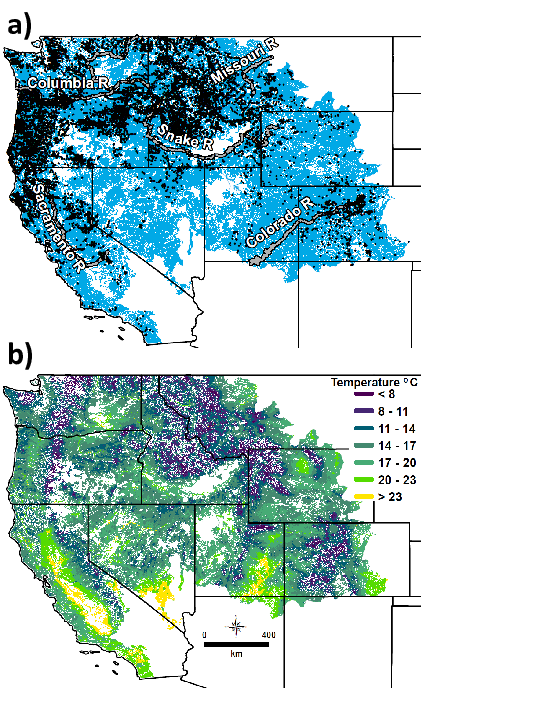
\includegraphics[width=0.9\linewidth]{/media/jay/Hitachi2GB/00NMML/ActiveBooks/SpatialStreamNetworks/_bookdown_files/SpatStatStreamNet_files/figure-html/Fig-Blob} 

}

\caption{a) Locations of temperature records measured with sensors at $>$20,000 unique stream sites in the NorWeST database, where the blue lines are streams, and the solid black circles are locations. b) Mean August temperature predictions throughout most of the western United States using methods described in this book.}\label{fig:Fig-Blob}
\end{figure}

Based on leave-one-out crossvalidation there was an \(r^2\) of 0.90
between true and predicted temperature values at observed sites, with a
root-mean-squared prediction error (RMSPE) of 1.0\(^0\)C across all
streams. The accuracy of the SSN temperature model used to develop the
scenarios, and the model's ability to extract reliable information from
large, non-random datasets collected by the management community, has
led to the rapid adoption and broad use of NorWeST scenarios for
conservation planning. The scenarios have been used to precisely
identify climate refugia for cold-water fishes such as trout and char
\citep{Isaa:Youn:Nage:Hora:Groc:2015:cold, Isaa:Youn:Luce:Host:slow:2016},
characterize thermal niches of fish and amphibian species
\citep{Al:Schm:Clan:Saff:Kova:others:brow:2016, Isaa:Weng:Youn:big:2017},
describe how salmon migrations are affected by temperature
\citep{West:Ditt:Ward:Quin:sign:2015}, and estimate the distribution and
abundance of fish populations
\citep{Dauw:Fese:Bjor:Usin:2015, Isaa:Ver:Pete:Hora:Nage:scal:2017}.

To illustrate statistical methods for stream networks in this Chapter,
we use a very small subset of the NorWeST data. The stream network and
sampling locations for the example are shown in Figure
\ref{fig:Fig-StudyArea}

\begin{figure}[h]

{\centering 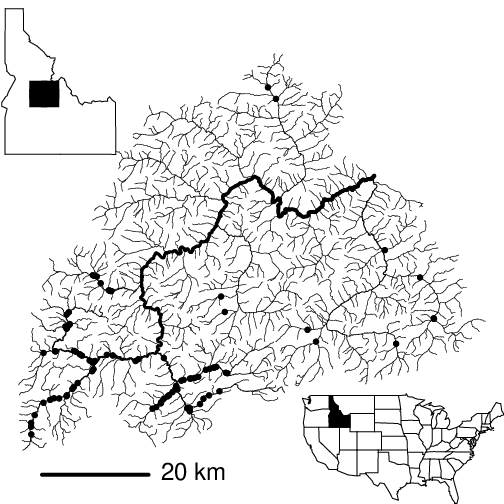
\includegraphics[width=0.7\linewidth]{/media/jay/Hitachi2GB/00NMML/ActiveBooks/SpatialStreamNetworks/_bookdown_files/SpatStatStreamNet_files/figure-html/StudyArea} 

}

\caption{The study area in central Idaho, where average August temperature data were collected from the Middle Fork of the Salmon River in 2004. The sample locations are shown as solid black circles.}\label{fig:Fig-StudyArea}
\end{figure}

\hypertarget{why-stream-network-models}{%
\section{Why Stream Network Models?}\label{why-stream-network-models}}

Many researchers have called for using stream distance, rather than
Euclidean distance, when developing spatial statistical models for
stream networks
\citep{Dent:Grim:spat:1999, Torg:Gres:Bate:patt:2004, Yuan:usin:2004}.
There is a problem, however, if we simply use stream distance, rather
than Euclidean distance, in a standard geostatistical autocovariance
model \citep[e.g., a large number geostatistical models based on
Euclidean distance can be found in][p.~80--97]{Chil:Delf:geos:1999}. To
illustrate, we computed stream distances between all pairs of stream
locations shown in Figure \ref{fig:Fig-StudyArea}, and then used stream
distances (rather than Euclidean distances) in five commonly-used
autocovariance models from geostatistics. For all 5 models, the
``nugget'' effect was set to zero and the ``partial sill'' was set to 1.
The parameter that controls the amount of autocorrelation, often called
the ``range,'' was allowed to vary. For each value of the range for each
model, a spatial covariance matrix was determined based on stream
distance among the 90 locations in Figure \ref{fig:Fig-StudyArea}. The
minimum eigenvalue as a function of the range is shown in Figure
\ref{fig:Fig-testEucValid}.

\begin{figure}[h]

{\centering 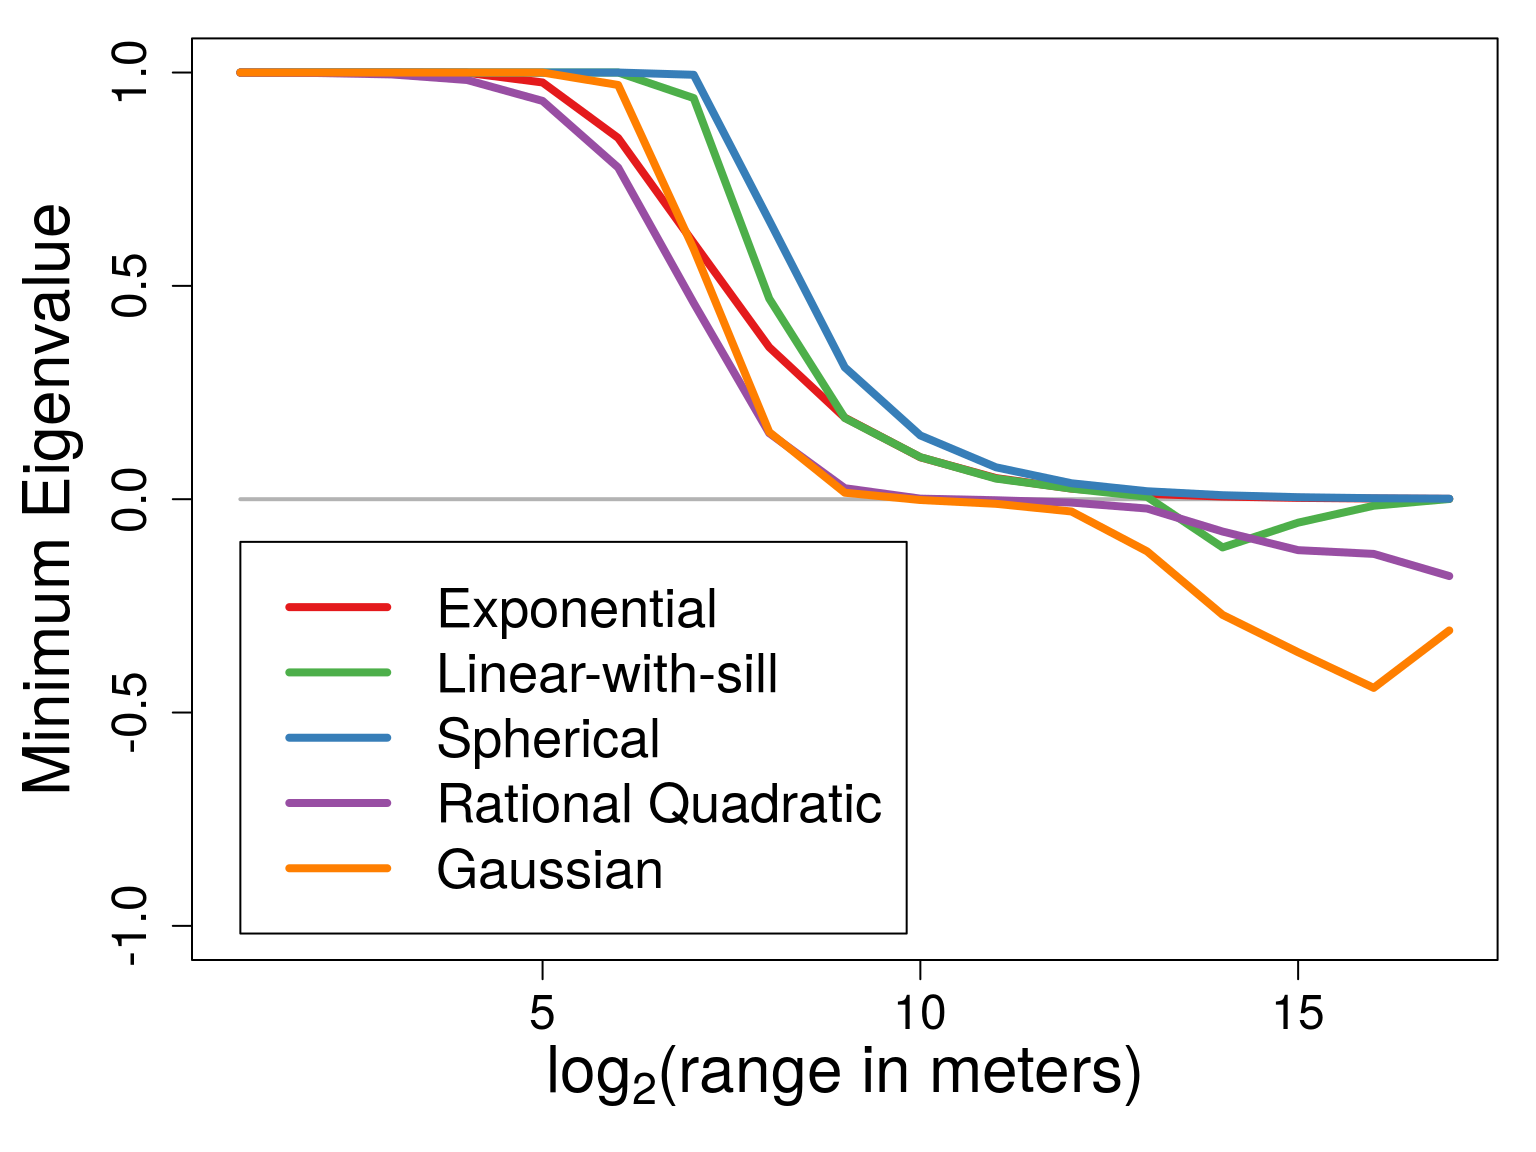
\includegraphics[width=0.7\linewidth]{SpatStatStreamNet_files/figure-latex/Fig-testEucValid-1} 

}

\caption{Minimum eigenvalues of spatial covariance matrices for classic geostatistical models based on Euclidean distances, for various range parameters (in log base 2 meters), but when using using stream distance, rather than Euclidean distance, among all locations shown in the Study Area Figure}\label{fig:Fig-testEucValid}
\end{figure}

Notice that negative eigenvalues mean that the covariance matrix is not
positive definite, and hence not valid. Figure
\ref{fig:Fig-testEucValid} demonstrates that the linear-with-sill,
rational quadratic, and Gaussian models are not valid when using stream
distance for this data set for certain range values. This illustrates
that simple substitution of stream network distance for Euclidean
distance does not guarantee valid models, in the sense that the
covariance matrix is not guaranteed to be positive definite. Even when a
model appears to be valid for all range values for a given data set,
such as the exponential or spherical models in Figure
\ref{fig:Fig-testEucValid}, there is no guarantee that additional
points, e.g.~for prediction purposes, will keep covariance matrices
positive definite. Similarly, a change in network configuration could
cause these models to fail; indeed, \citet{Ver:Pete:Theo:spat:2006} show
a network where the spherical model has negative eigenvalues. Despite
this, some researchers continue to erroneously substitute network
distance into models designed for geostatistics. Thus, in order to use
stream distance rather than Euclidean distance, another approach is
indicated.

Even though substituting stream distance for Euclidean distance does not
guarantee valid models, it is fair to ask why use stream distance at
all? Fitting SSN models requires more effort than fitting standard
geostatistical methods. Calculating stream distances, and weighting
stream segments (as we will describe below) requires considerable GIS
computation, whereas Euclidean distance can be readily calculated in R
(or any software) without a GIS. What is gained by the stream network
models? Consider a simple example using the data in Figure
\ref{fig:Fig-StudyArea}. We withheld one measurement, the open circle in
Figure \ref{fig:Fig-whyStreamNet}, which also shows its two closest
locations (solid circles).

\textbackslash{}begin\{figure\}{[}h{]}

\{\centering 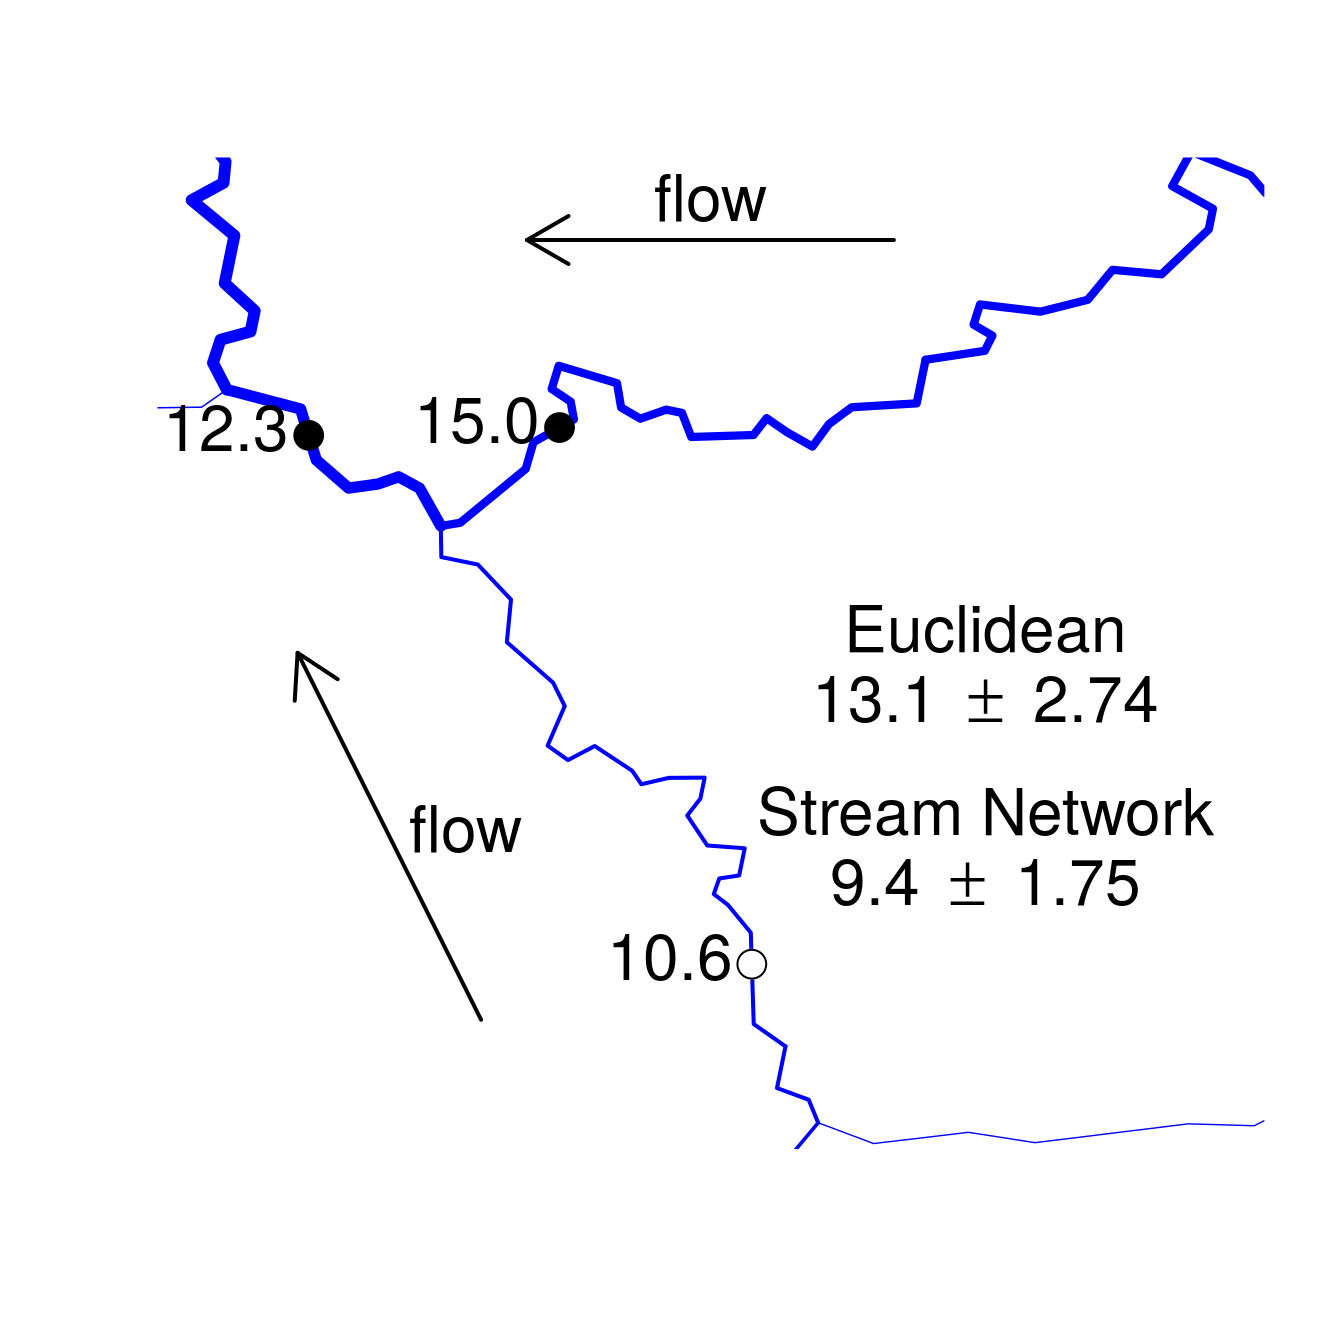
\includegraphics[width=0.7\linewidth]{SpatStatStreamNet_files/figure-latex/Fig-whyStreamNet-1}

\}

\textbackslash{}caption\{A comparison of ordinary kriging predictions,
using a covariance matrix based on Euclidean distance, and predictions
from a stream network model, using a covariance matrix based on stream
distance and flow information. The values at the solid circles are used
as observed data to predict the value at the open circle. The real value
at the open circle is given, along with predictions for the two models
with 90\% prediction invervals.\}\label{fig:Fig-whyStreamNet}
\textbackslash{}end\{figure\}

We predicted the withheld observation using ordinary kriging
\citep{Cres:stat:1993} based on Euclidean distance, and also predicted
it based on a stream-network model \citep{Ver:Pete:Move:2010} that we
will discuss in greater detail below. Ordinary kriging, based on
Euclidean distance, predicted a value for the withheld location of
13.1\(^{\circ}\)C, with a 90\% prediction interval of \(\pm\)
2.74\(^{\circ}\)C. A tail-up stream-network model predicted a lower
value of 9.4\(^0\)C, with a prediction interval of \(\pm\)
1.75\(^{\circ}\)C. Both intervals capture the true value, but the stream
network prediction is more accurate. However, there is more of interest.
Recall that ordinary kriging generally weights nearby locations most
heavily, and the prediction, 13.1, is somewhere between observed values
12.3 and 15.0. From this perspective, the Euclidean model produces a
sensible prediction (Figure \ref{fig:Fig-whyStreamNet}). Yet, this is
not logically consistent for a flowing stream. Notice that the
temperature decreased from 15.0\(^{\circ}\)C to 12.3\(^{\circ}\)C
downstream between the two observed locations on the main stream segment
(thicker line), even though temperature generally increases while going
downstream. This suggests that the unobserved tributary added cold
water, causing the drop in temperature. Logically, the downstream
temperature of 12.3\(^{\circ}\)C should be some weighted average of
temperatures from the two upstream segments; one with a temperature of
15.0\(^{\circ}\)C, and while the other temperature is unknown, it is
surely less than 12.3\(^{\circ}\)C. Thus, the ordinary kriging estimate
of 13.1\(^{\circ}\)C is not logically consistent, whereas the estimate
from the stream-network model, 9.4\(^{\circ}\)C, is logically
consistent. Although this is but a single prediction, we have observed
this type of difference between ordinary kriging and stream network
model predictions on many occasions, where the stream network model
tends to reflect the topological constraints and the effect of flow on
correlation structure. A similar example is given by
\citet{Pete:Ver:Isaa:stre:2013}.

\hypertarget{topology-and-distance}{%
\chapter{Topology and Distance}\label{topology-and-distance}}

\hypertarget{topology}{%
\section{Topology}\label{topology}}

We define stream segments as lines between junctions in a stream network
\citep{Ver:Pete:Theo:spat:2006, Ver:Pete:Move:2010}. Our convention is
that a location downstream is assigned a lower real number for position
than a location upstream. A dendritic stream network has a single
most-downstream point (the outlet), which we set to 0, and it is the
point from which all distances are computed. We define ``distance
upstream'' to be the length of the line from any location on a stream
network that can be connected by a continuous line to the network outlet
(lowest point in that network). For model development it will be
convenient to extend all terminal upstream segments to \(\infty\) and a
line downstream of the outlet to \(-\infty\).

There are a finite number of stream segments in an SSN, and we index
them arbitrarily with \(i = 1,2,\ldots\). Many locations will have the
same distance from the outlet (our 0 point) in an SSN, so to uniquely
define locations using distance upstream, we denote locations as
\(x_i\), where \(x\) is distance upstream and \(i\) indicates that it is
on the \(i\)th stream segment. In Figure \ref{fig:Fig3SegStream},
\(r_1\) is distance \(r\) upstream and it is located on the segment
labeled 1. Note the arbitrary labeling of segments \(r_1\), \(s_2\), and
\(t_3\) as seen in Figure \ref{fig:Fig3SegStream}. We use \(l_i\) for
the smallest, and \(u_i\) for the largest, upstream distance on the
\(i\)th segment (Figure \ref{fig:Fig3SegStream}).

\begin{figure}[h]

{\centering 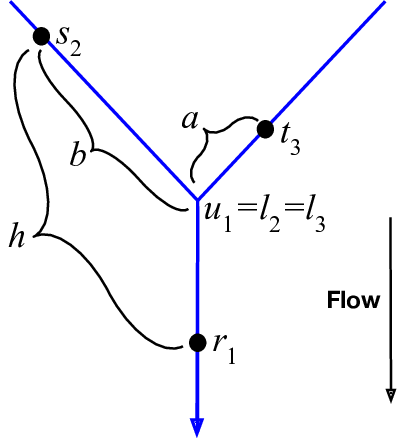
\includegraphics[width=0.6\linewidth]{/media/jay/Hitachi2GB/00NMML/ActiveBooks/SpatialStreamNetworks/_bookdown_files/SpatStatStreamNet_files/figure-html/Fig3SegStream} 

}

\caption{Three locations on a stream network, $r_1$, $s_2$, $t_3$.  The location of the farthest upstream distance on segment 1 is $u_1$.  The locations of the farthest downstream distances on segments 2 and 3 are $l_2$ and $l_3$, respectively.  Effectively, $u_1 = l_2 = l_3$, but it is convenient to use the distinct notation. For FU sites ($s_2$ and $t_3$), $a$ is used for the shorter distance to their common junction, and $b$ is used for the longer distance.  When sites are FC ($s_2$ and $r_1$), $h$ is used to denote the distance between them.}\label{fig:Fig3SegStream}
\end{figure}

Let \(A\) be the set of all stream segment indices. We denote \(U_{i}\),
a subset of \(A\), as the set of stream segments upstream of \(x_i\),
including the \(i\)th segment, and we denote \(U^{*}_{i}\) as the set
excluding the \(i\)th segment. We denote \(D_{i}\), also a subset of
\(A\), as the set of stream segments downstream of \(x_i\), including
the \(i\)th segment, and we denote \(D^{*}_{i}\) as the set excluding
the \(i\)th segment. This notation make precise the definition of
``flow-connected'' (FC) for two locations, \(r_i\) and \(s_j\), if
\(U_i \cap U_j \neq \emptyset\), and they are ``flow-unconnected'' (FU)
if \(U_i \cap U_j = \emptyset\). We can also define the set of stream
segments ``between'' two FC locations, \(r_i \leq s_j\), exclusive of
the \(i\)th and \(j\)th segments, as \(D^{*}_{j} \setminus D_i\). For
point locations, we use \(\vee_s\) to denote the network only upstream
of point \(s\), including all branchings, and \(\wedge_s\) to denote the
network downstream of \(s\) that follows flow only (i.e., it does not go
downstream and then back upstream).

Modeling covariance requires total stream distance between pairs of
points, so for two FU locations we will use \(a\) to indicate the
shorter distance from one location to the nearest junction downstream
that shares flow with the other location (\ref{fig:Fig3SegStream}), and
we use \(b\) to indicate the longer distance to the same junction. We
use \(h\) for the distance between two FC locations (Figure
\ref{fig:Fig3SegStream}.

\hypertarget{fast-computing-for-distances-in-a-branching-network}{%
\section{Fast Computing for Distances in a Branching
Network}\label{fast-computing-for-distances-in-a-branching-network}}

In general, a straightforward approach for keeping track of network
structure in a directed graph, such as a stream network, is to label
segments (we adopt the graph terminology ``edge''). A ForwardStar data
structure \citep{Ahuj:Magn:Orli:netw:1993} is commonly used to keep
track of which edge leads to another edge. This data structure is based
on a set of ``to-from'' tables, which store information about the
coincidence of features and can be searched to generate new spatial
information. However, traversing to-from tables generated from a large
stream network is computationally intensive, especially in an
interpreted programming language like \textbf{R}. As an alternative, we
developed a system based on a binary identifier (ID), which is used to
rapidly assess flow-connectivity and stream distance between any two
locations on the dendritic stream network.

The process of assigning binary IDs is conceptually simple. First, the
outlet edge (i.e., the most downstream edge in the network) is
identified and assigned a binary ID equal to 1 (Figure
\ref{fig:FigBinaryID}). The information stored in the to-from table is
then used to identify edges that are directly upstream from the outlet
edge. Binary IDs are assigned to the upstream edge(s) by arbitrarily
appending a 0 or 1 to the downstream binary ID. For example, binary IDs
10 and 11 are directly upstream from binary ID 1 in Figure
\ref{fig:FigBinaryID}. This process of moving upstream and assigning
binary IDs continues until every edge in the stream network has been
assigned a binary ID. Note that the binary ID is only unique within a
stream network. Also, the binary ID is not the binary number that is
equivalent to the segment number. Stream segments are numbered
arbitrarily and sequentially, but binary IDs actually represent the
branching structure.

\begin{figure}[h]

{\centering 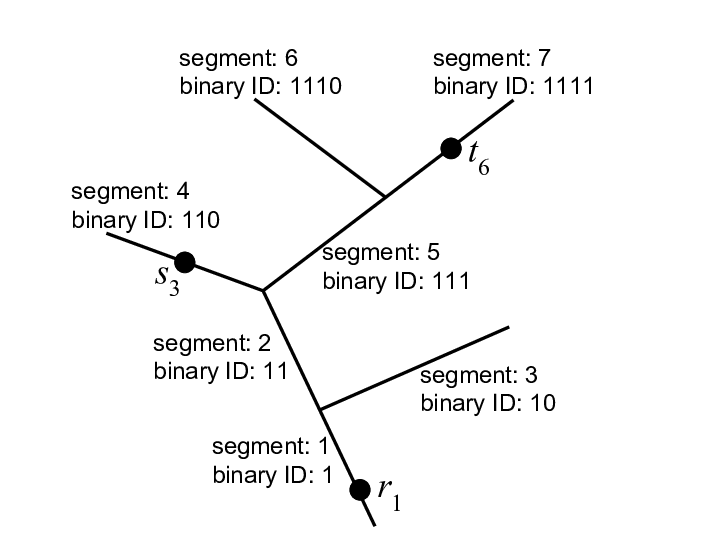
\includegraphics[width=0.7\linewidth]{/media/jay/Hitachi2GB/00NMML/ActiveBooks/SpatialStreamNetworks/_bookdown_files/SpatStatStreamNet_files/figure-html/FigBinaryID} 

}

\caption{A binary identifier (ID) is assigned to each segment in a stream network.  Use of binary IDs allows rapid assessment of flow-connectedness, distance to junctions, and stream distance among points on the network.}\label{fig:FigBinaryID}
\end{figure}

The binary IDs are useful because they provide a way to rapidly
determine whether locations have an FC or FU relationship. Two locations
are considered FC when water flows from an upstream location to a
downstream location. In contrast, two locations are FU when they reside
on the same network, but water does not flow between them. In Figure
\ref{fig:FigBinaryID}, site \(r_1\) resides on the most downstream
segment in the network (segment 1). Thus, the binary ID for \(r_1\) is
completely nested within the binary ID for the edge containing site
\(s_3\) (``1'' is nested within ``110''), which indicates that the two
locations are FC. If the binary IDs for two edges are not nested, as is
the case for \(s_3\) and \(t_6\) (``110'' is not nested within
``1111''), the two locations are FU. In addition, the binary IDs for FU
locations contain information about the closest common downstream
location. As an example, the most common downstream junction between
sites \(s_3\) and \(t_6\) is ``11'' (Figure \ref{fig:FigBinaryID}) and
so ``11'' is the binary ID of the stream segment where sites \(s_3\) and
\(t_6\) diverge.

One of the advantages of SSN models is that they can be used to
represent both FC and FU relationships within a stream network. In order
to do this, information about directional relationships must be
preserved within an asymmetric distance matrix, which contains the
downstream-only distance between each pair of locations. Four pieces of
spatial information are generated using the STARS toolset and
subsequently used to calculate the downstream-only stream distance
matrix: 1) the network ID, 2) the binary IDs, 3) the upstream distance
from the network outlet to the most upstream location on each edge,
\(u_i\) and 4) the upstream distance from the outlet to each location,
\(x_i\). As mentioned previously, the binary IDs are only unique within
a network and so the first step is to determine whether two locations
reside on the same network using the network IDs. When this is true, the
binary IDs are used to determine whether two locations are FC or FU. If
they are FU, the downstream-only distance between \(t_3\) and \(s_2\)
(Figure \ref{fig:Fig3SegStream}), \(a\), is \(t_3 - u_1\), while the
downstream-only distance between \(s_2\) and \(t_3\), \(b\), is
\(s_2 - u_1\). For FC sites, again determined by the binary IDs, the
downstream-only distance from \(s_2\) to \(r_1\) is \(s_2-r_1>0\), while
\(r_1-s_2=0\). In fact, for any set of \(n\) locations, the directional
distances can be stored in an asymmetric \(n \times n\) matrix, which
stores the distance to the common junction. In addition, the total
stream distance between locations is generated by adding the transpose
of the \(n \times n\) matrix, to itself. Thus, everything required to
construct the models described below is contained in this asymmetric
matrix.

\hypertarget{theory}{%
\chapter{Theory}\label{theory}}

\hypertarget{moving-average-models}{%
\section{Moving Average Models}\label{moving-average-models}}

\citet{Yagl:corr:1987}\} shows that a large class of autocovariances can
be developed by creating random variables as the integration of a
moving-average function over a white-noise random process,

\begin{equation} 
    Z(s;\boldsymbol{\theta}) = \int_{-\infty}^{\infty}g(x-s;\boldsymbol{\theta})dW(x),
    \label{eq:Zdef}
\end{equation}

where \(x\) and \(s\) are locations on the real line,
\(g(x;\boldsymbol{\theta})\) is called the moving-average function
defined on \(\mathcal{R}^{1}\) and is square-integrable, and recall that
when \(W(x)\) is Brownian motion,

\[
E[Z(s;\boldsymbol{\theta})^2]=\int_{-\infty}^{\infty}g(x;\boldsymbol{\theta})^2dx.
\]

The moving-average construction \eqref{eq:Zdef} allows a valid
autocovariance between \(Z(s)\) and \(Z(s+h)\) to be expressed as

\begin{equation} 
    C(h;\boldsymbol{\theta})= 
        \int_{-\infty}^{\infty}g(x;\boldsymbol{\theta})g(x-h;\boldsymbol{\theta})dx.
\label{eq:moveave}
\end{equation}

\hypertarget{tail-up-models}{%
\section{Tail-up Models}\label{tail-up-models}}

The moving average construction in \eqref{eq:Zdef} and \eqref{eq:moveave} is
well-known for the continuous real line from \(-\infty\) to \(\infty\),
such as for time-series models. \citet{Ver:Pete:Theo:spat:2006} and
\citet{Cres:Frey:Harc:Smit:spat:2006} use moving averages for a stream
network to develop models as in

\hypertarget{applications}{%
\chapter{Applications}\label{applications}}

Some \emph{significant} applications are demonstrated in this chapter.

\hypertarget{example-one}{%
\section{Example one}\label{example-one}}

\hypertarget{example-two}{%
\section{Example two}\label{example-two}}

\hypertarget{final-words}{%
\chapter{Final Words}\label{final-words}}

We have finished a nice book.

\bibliography{book.bib,packages.bib,jss984.bib,StatBibTex.bib}


\end{document}
